The same held-out users and 10,833 prediction targets are used for every method in Table~\ref{tab:compact-results}. Fitted neural models and the adaptive ensemble report the mean of seeds 11, 23, and 37. In descending Top-3 order, the proposed variants are UNCP 5 (85.09\%), UNCP 6 (84.08\%), UNCP 2 (83.58\%), UNCP (82.30\%), UNCP 3 (81.40\%), and UNCP 4 (81.08\%). The table is ordered by increasing Top-3 accuracy so that the highest result appears last. UNCP 5's paired gain over UNCP 2 is 1.51 percentage points, with an exploratory user-cluster bootstrap interval of 1.03--1.77 points over 11 held-out users. Gate coefficients were selected only on validation users.

\newcommand{\modeldetail}[1]{{\footnotesize\color{uncptealdark}(#1)}}
\newcommand{\score}[2]{#1\,{\color{black!55}\scriptscriptstyle\pm\,#2}}
\newcommand{\uncpbase}{UNCP \modeldetail{GRU--Transformer fusion}}
\newcommand{\uncptwo}{UNCP 2 \modeldetail{transition-graph-aware GRU--Transformer}}
\newcommand{\uncpthree}{UNCP 3 \modeldetail{GRU, Transformer, Mamba-2-inspired SSD}}
\newcommand{\uncpfour}{UNCP 4 \modeldetail{typed graph attention, GRU, transition graph, candidate masking, adaptive fusion}}
\newcommand{\uncpfive}{\textbf{UNCP 5} \modeldetail{UNCP 2, transition model, adaptive fusion}}
\newcommand{\uncpsix}{UNCP 6 \modeldetail{dual GRU streams, run lengths, repeat/switch head}}

\begin{table}[!htbp]
\centering
\caption{Held-out account comparison, sorted by increasing Top-3 accuracy (percent; fitted models report mean $\pm$ sample SD over three seeds).}
\label{tab:compact-results}
\small
\begin{tabular}{@{}p{.53\linewidth}rr@{}}
\toprule
Model & Top-1 & Top-3 \\
\midrule
Uniform expected & 1.10 & 3.30 \\
Global popularity & 5.16 & 22.37 \\
Logistic regression & $\score{44.24}{0.61}$ & $\score{71.58}{0.33}$ \\
Transformer & $\score{44.46}{0.52}$ & $\score{71.92}{0.36}$ \\
RNN & $\score{50.22}{0.26}$ & $\score{75.10}{0.48}$ \\
LSTM & $\score{54.52}{0.06}$ & $\score{78.00}{0.55}$ \\
GRU & $\score{55.97}{0.62}$ & $\score{78.88}{0.40}$ \\
Markov-4 & 60.27 & 79.91 \\
\uncpfour & $\score{59.84}{1.40}$ & $\score{81.08}{0.88}$ \\
\uncpthree & $\score{61.12}{2.29}$ & $\score{81.40}{0.82}$ \\
\uncpbase & $\score{62.72}{0.95}$ & $\score{82.30}{0.52}$ \\
\uncptwo & $\score{64.62}{1.10}$ & $\score{83.58}{0.04}$ \\
\uncpsix & $\score{66.60}{0.51}$ & $\score{84.08}{0.22}$ \\
\uncpfive & $\mathbf{\score{66.71}{0.84}}$ & $\mathbf{\score{85.09}{0.20}}$ \\
\bottomrule
\end{tabular}
\end{table}

\begin{figure}[!htbp]
\centering
\begin{tikzpicture}
\begin{axis}[ybar,width=.98\linewidth,height=5.3cm,ymin=0,ymax=100,
symbolic x coords={Logistic,Transformer,RNN,LSTM,GRU,Markov4,UNCP4,UNCP3,UNCP,UNCP2,UNCP6,UNCP5},
xtick=data,x tick label style={rotate=35,anchor=east,font=\scriptsize},
ytick={0,20,40,60,80,100},ylabel={Accuracy (\%)},
bar width=5pt,legend style={at={(.5,1.02)},anchor=south,legend columns=2,font=\small},
enlarge x limits=.08]
\addplot[fill=gray!55] coordinates {(Logistic,44.24)(Transformer,44.46)(RNN,50.22)(LSTM,54.52)(GRU,55.97)(Markov4,60.27)(UNCP4,59.84)(UNCP3,61.12)(UNCP,62.72)(UNCP2,64.62)(UNCP6,66.60)(UNCP5,66.71)};
\addplot[fill=uncpteal] coordinates {(Logistic,71.58)(Transformer,71.92)(RNN,75.10)(LSTM,78.00)(GRU,78.88)(Markov4,79.91)(UNCP4,81.08)(UNCP3,81.40)(UNCP,82.30)(UNCP2,83.58)(UNCP6,84.08)(UNCP5,85.09)};
\legend{Top-1,Top-3}
\end{axis}
\end{tikzpicture}
\caption{Updated Top-1 and Top-3 comparison on the user-disjoint test set. Values are generated directly from the verified result files.}
\label{fig:updated-accuracy}
\end{figure}

Table~\ref{tab:protocol-results} provides the second and final result table. The temporal subset is a separate robustness analysis with a different eligible cohort, not a directly comparable improvement over the user-disjoint split. UNCP 2--6 have not been evaluated on that subset; their temporal cells are intentionally left unreported. The figure retains the visual comparison used in the original article while replacing the historical contaminated-split scores with the new protocol results.

\begin{table}[!htbp]
\centering
\caption{Top-3 accuracy under two leakage-aware protocols, ordered by increasing held-out-user accuracy (percent). A dash denotes an unrun temporal experiment.}
\label{tab:protocol-results}
\small
\begin{tabular}{@{}p{.53\linewidth}rr@{}}
\toprule
Model & Held-out users & Temporal subset \\
\midrule
Transformer & 71.92 & 73.59 \\
RNN & 75.10 & --- \\
LSTM & 78.00 & 83.84 \\
GRU & 78.88 & 84.74 \\
Markov-4 & 79.91 & 88.15 \\
\uncpfour & 81.08 & --- \\
\uncpthree & 81.40 & --- \\
\uncpbase & 82.30 & \textbf{89.95} \\
\uncptwo & 83.58 & --- \\
\uncpsix & 84.08 & --- \\
\uncpfive & \textbf{85.09} & --- \\
\bottomrule
\end{tabular}
\end{table}

\begin{figure}[!htbp]
\centering
\begin{subfigure}{.49\linewidth}
\centering
\begin{tikzpicture}
\begin{axis}[ybar,width=\linewidth,height=4.4cm,ymin=0,ymax=100,
symbolic x coords={Transformer,RNN,LSTM,GRU,Markov4,UNCP4,UNCP3,UNCP,UNCP2,UNCP6,UNCP5},xtick=data,
x tick label style={rotate=45,anchor=east,font=\tiny},ytick={0,25,50,75,100},
title={Held-out users},title style={font=\small},bar width=10pt,enlarge x limits=.12]
\addplot[fill=uncpteal] coordinates {(Transformer,71.92)(RNN,75.10)(LSTM,78.00)(GRU,78.88)(Markov4,79.91)(UNCP4,81.08)(UNCP3,81.40)(UNCP,82.30)(UNCP2,83.58)(UNCP6,84.08)(UNCP5,85.09)};
\end{axis}
\end{tikzpicture}
\end{subfigure}
\begin{subfigure}{.49\linewidth}
\centering
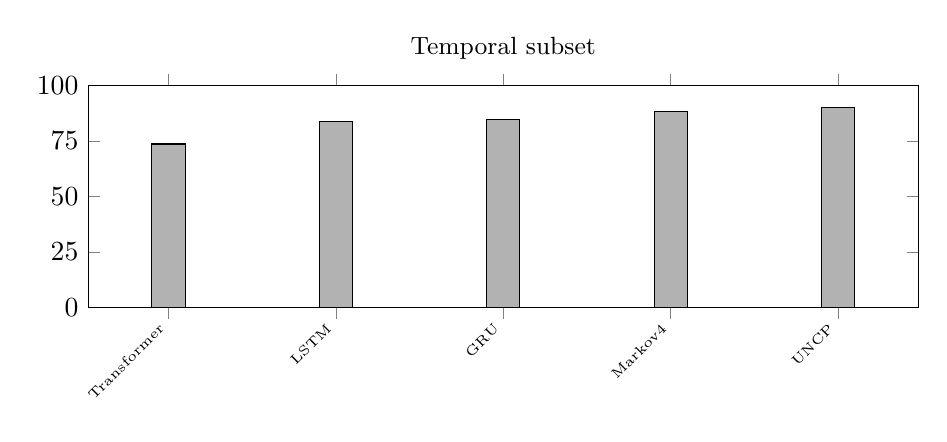
\begin{tikzpicture}
\begin{axis}[ybar,width=\linewidth,height=4.4cm,ymin=0,ymax=100,
symbolic x coords={Transformer,LSTM,GRU,Markov4,UNCP},xtick=data,
x tick label style={rotate=45,anchor=east,font=\tiny},ytick={0,25,50,75,100},
title={Temporal subset},title style={font=\small},bar width=12pt,enlarge x limits=.12]
\addplot[fill=gray!60] coordinates {(Transformer,73.59)(LSTM,83.84)(GRU,84.74)(Markov4,88.15)(UNCP,89.95)};
\end{axis}
\end{tikzpicture}
\end{subfigure}
\caption{Top-3 accuracy for selected models under the held-out-user and qualified temporal protocols.}
\label{fig:updated-protocols}
\end{figure}

Top-1 requires the observed next click to be the highest-ranked prediction, whereas Top-3 counts success when it appears among the three highest scores. Both are reported because Top-3 is useful for ranking candidate interactions, but it must be interpreted alongside transparent baselines and the candidate space. Numerical comparisons with other publications are not used to claim superiority because their datasets, interfaces, labels, and split procedures differ.
